\input ../SlidePreamble
\input ../preamble

\begin{document}

{\Huge

  \centerline{\bf TTIC 31230, Fundamentals of Deep Learning}
  \bigskip
  \centerline{David McAllester, Winter 2020}
  \vfill
  \centerline{\bf Language Modeling}
  \vfill
  \centerline{\bf Recurrent Nerual Networks (RNNs)}
  \vfill
  \centerline{\bf Machine Translation}

\slide{Natural Language Understanding}

GLUE: General Language Understanding Evaluation

\vfill

\centerline{\normalsize ArXiv 1804.07461}
\centerline{\includegraphics[width= 7in]{\images/GLUE}}

\slide{BERT and GLUE}

\centerline{\includegraphics[width= 7in]{\images/GLUELeader}}

\slide{BERT and SuperGLUE}

\centerline{\includegraphics[width= 9in]{\images/SuperLeader}}

\slide{ Language Modeling}

The recent progress on NLP benchmarks is due to pretraining on language modeling.

\vfill
Langauge modeling is based on unconditional cross-entropy minimiztion.

\vfill
$$\Phi^* = \argmin_\Phi \;E_{y \sim \pop}\;-\ln Q_\Phi(y)$$

\vfill
In language modeling $y$ is a sentence (or fixed length block of text).

\slide{Autoregressive Models}

A structured object, such as a sentence or an image, has an exponentially small probability.

\vfill
An autoregressive model computes conditional probability for each part given ``earlier'' parts.

\vfill
This can be done for the words of a sentence or the pixels of an image.

\vfill
Warning: BERT is not autoregressive.  But we will study autoregressive models first.

\slide{Langauge Modeling}

Let $W$ be some finite vocabulary of tokens (words).

\vfill
Let $\mathrm{Pop}$ be a population distribution over $W^*$ (sentences).

\vfill
We want to train a model $Q_\Phi(y)$ for sentences $y$

\begin{eqnarray*}
\Phi^* & = & \argmin_\Phi \; E_{y \sim \mathrm{Pop}}\;-\ln Q_\Phi(y)
\end{eqnarray*}

\slide{The End of Sentence Token {\tt <EOS>}}

We want to define a probability distribution over sentence of different length.

\vfill
For this we require that each sentence is ``terminated'' with an end of sentence token {\tt <EOS>}.

\vfill
We requite $w_T = \mbox{\tt <EOS>}$ and $w[t] \not = \mbox{\tt <EOS>}$ for $t < T$.

\vfill
This allows

$$P(w_0, w_1, \cdots, w_T) = \prod_{t=0}^T\;P(w_t\;|\;w_1,\ldots,w_{t-1})$$

To handle sentences of different length.


\slide{Recurrent Neural Network (RNN) Language Modeling}



\centerline{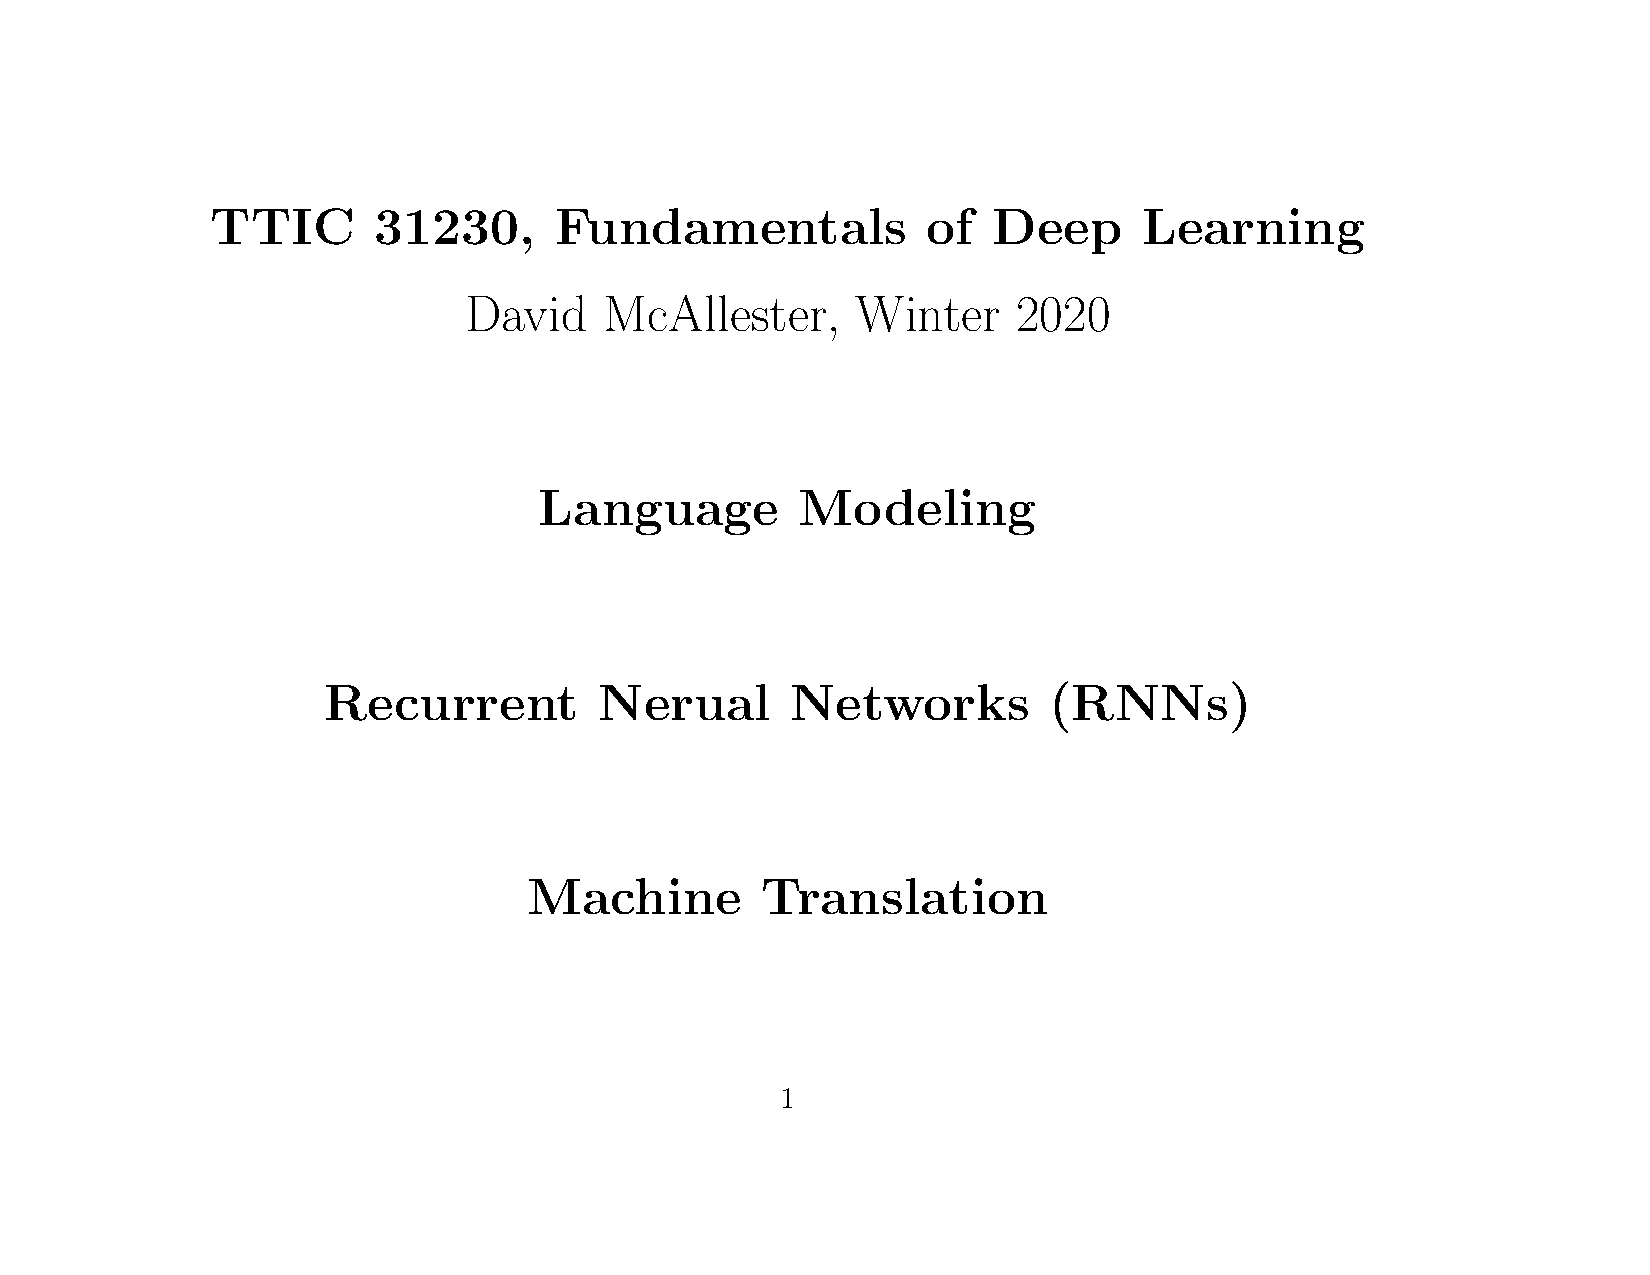
\includegraphics[width=3.5in]{../images/RNN}}
\centerline{{\large [Christopher Olah]}}

A typical neural language model has the form

$$Q_\Phi(w_t\;|\;w_1,\cdots,w_{t-1}) = \softmax_{w_t} e(w_t)^\top h_{t-1}$$

\vfill
{\bf Word Embeddings:} Here each word $w$ is associated with a vector $e(w)$ called the embedding of word $w$.


\slide{Standard Measures of Performance}

{\bf Bits per Character:}
For character language models performance is measured in bits per character.  Typical numbers are slightly over one bit per character.

\vfill
{\bf Perplexity:}
It would be natural to measure word language models in bits per word.  However, it is traditional to measure them in perplexity which is defined to be
$2^b$ where $b$ is bits per word.  Perplexities of about 60 were typical until the past couple years.  Today's large language models (ELMO, GPT-2) give
perplexities of about 30.

\vfill
According to Quora there are 4.79 letters per word.  1 bit per character (including space characters) gives a perplexity of $2^{5.79}$ or $55.3$.

\slide{}

\centerline{\bf Recurrent Neural Networks (RNNs)}

\slide{Review of Implicit Summation Notation}

Capital letter indeces are used to indicate subtensors (slices) so that, for example,  $M[I,J]$ denotes a matrix
while $M[i,j]$ denotes one element of the matrix, $M[i,J]$ denotes the $i$th row, and $M[I,j]$ denotes the $j$th collumn.

\vfill
We will adopt the convention, similar to true Einstein notation, that repeated capital indeces in a product of tensors are implicitly summed.  For example, we can write the inner product $e[w,I]^\top h[t,I]$ simply as $e[w,I]h[t,I]$ without the need for the (meaningless) transpose operation.

\slide{Vanilla RNNs}

\centerline{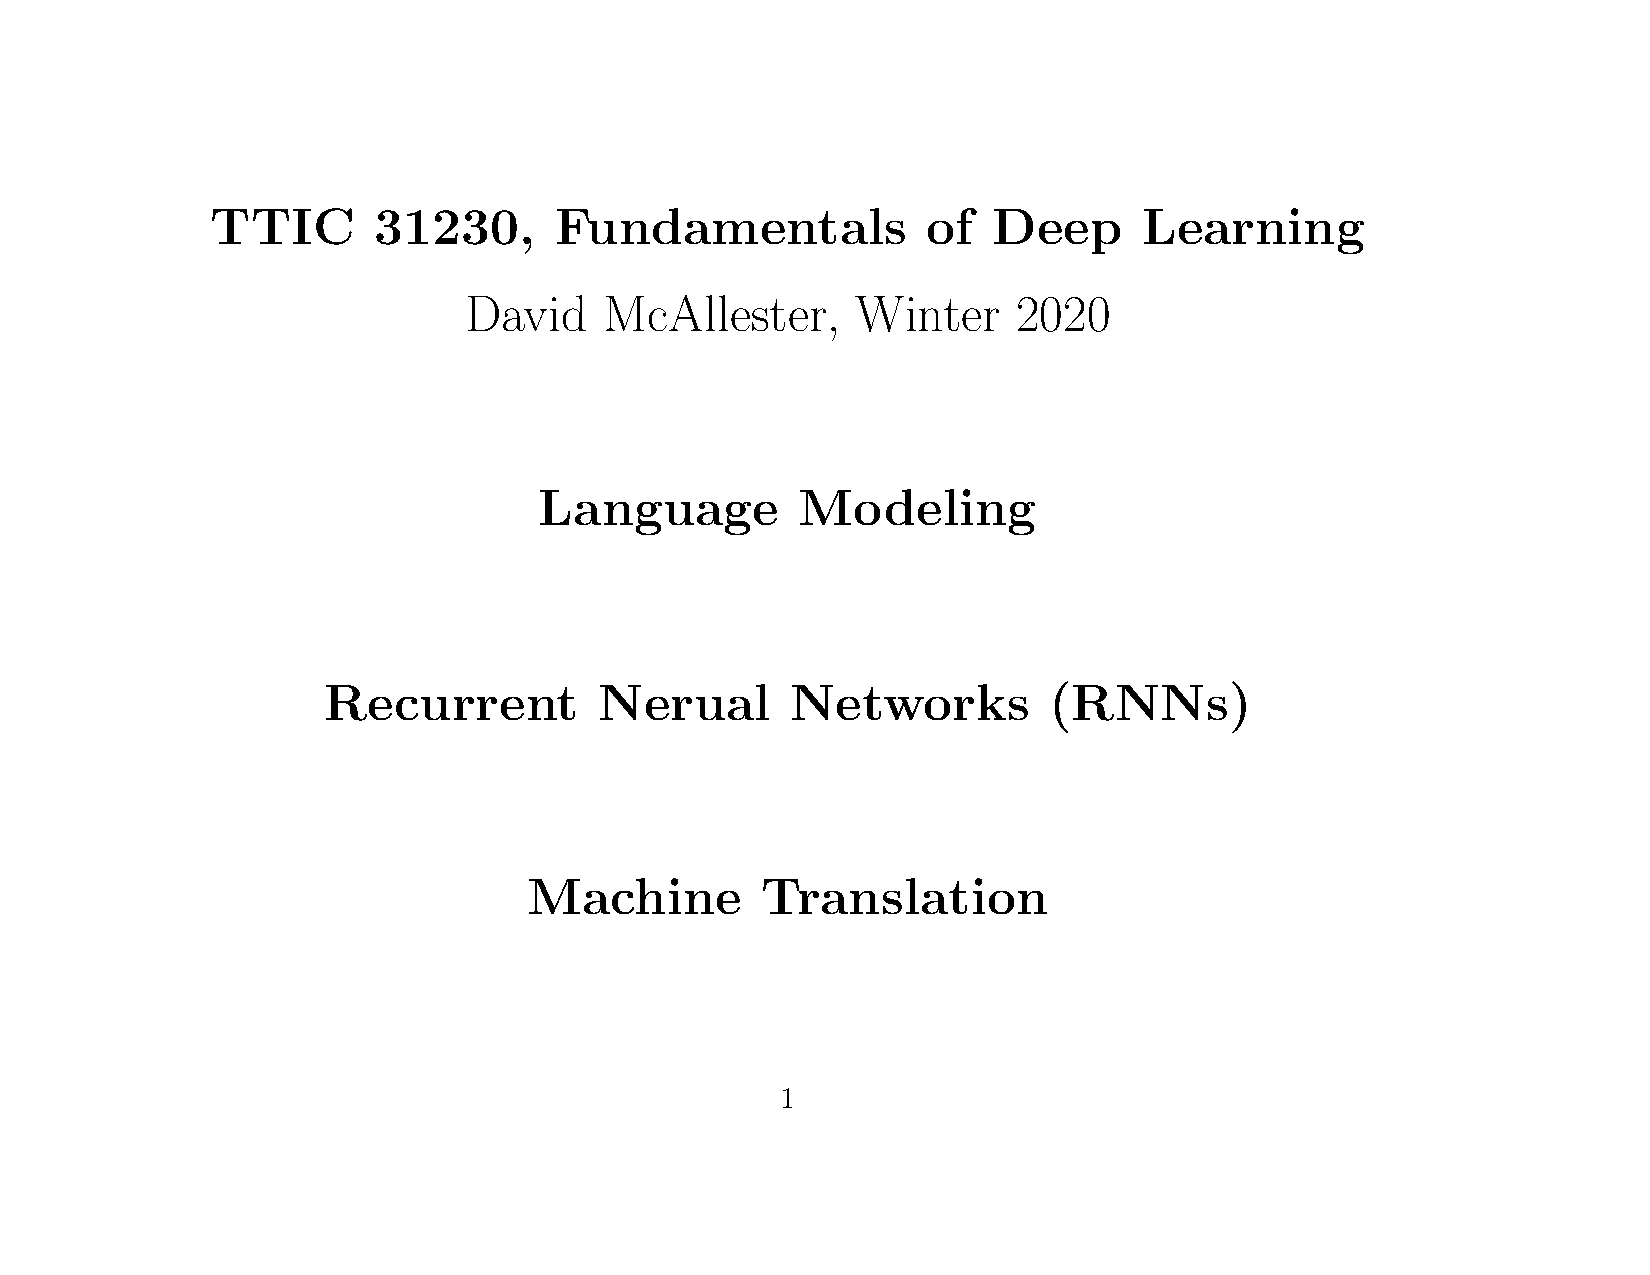
\includegraphics[width=3.5in]{../images/RNN}}
\centerline{{\large [Christopher Olah]}}

A Vanilla RNN uses two-input linear threshold units.

{\huge
\begin{eqnarray*}
& & {\color{red} h[b,t,j]} \\
\\
& = & \sigma\left(\left(\sum_i\;W^{h,h}[j,i]{\color{red} h[b,t-1,i]}\right) + \left(\sum_k W^{x,h}[j,k]{\color{red} x[b,t,k]}\right) - B[j]\right) \\
\\
\\
& = & \sigma\left(W^{h,h}[j,I]{\color{red} h[b,t-1,I]} + W^{x,h}[j,K]{\color{red} x[b,t,K]} - B[j]\right)
\end{eqnarray*}
}

\slideplain{Exploding and Vanishing Gradients}

\vfill
If we avoid saturation of the activation functions then we get exponentially growing or shrinking eigenvectors of the weight matrix.

\vfill
Note that if the forward values are bounded by sigmoids or tanh then they cannot explode.

\vfill
However the gradients can still explode.

\slide{Exploding Gradients: Gradient Clipping}

\vfill
We can dampen the effect of exploding gradients by clipping them before applying SGD.

\vfill
$$W.\mathrm{grad'} = \left\{\begin{array}{l} W.\mathrm{grad} \;\;\;\mbox{if $||W.\mathrm{grad}|| \leq n_{\mathrm{max}}$} \\
                                                      \\ \\
                                                      n_{\mathrm{max}} \; W.\mathrm{grad} / ||W.\mathrm{grad}|| \;\; \mbox{otherwise}
\end{array} \right.$$

\vfill
See {\tt torch.nn.utils.clip\_grad\_norm}

\slide{Time as Depth}

\centerline{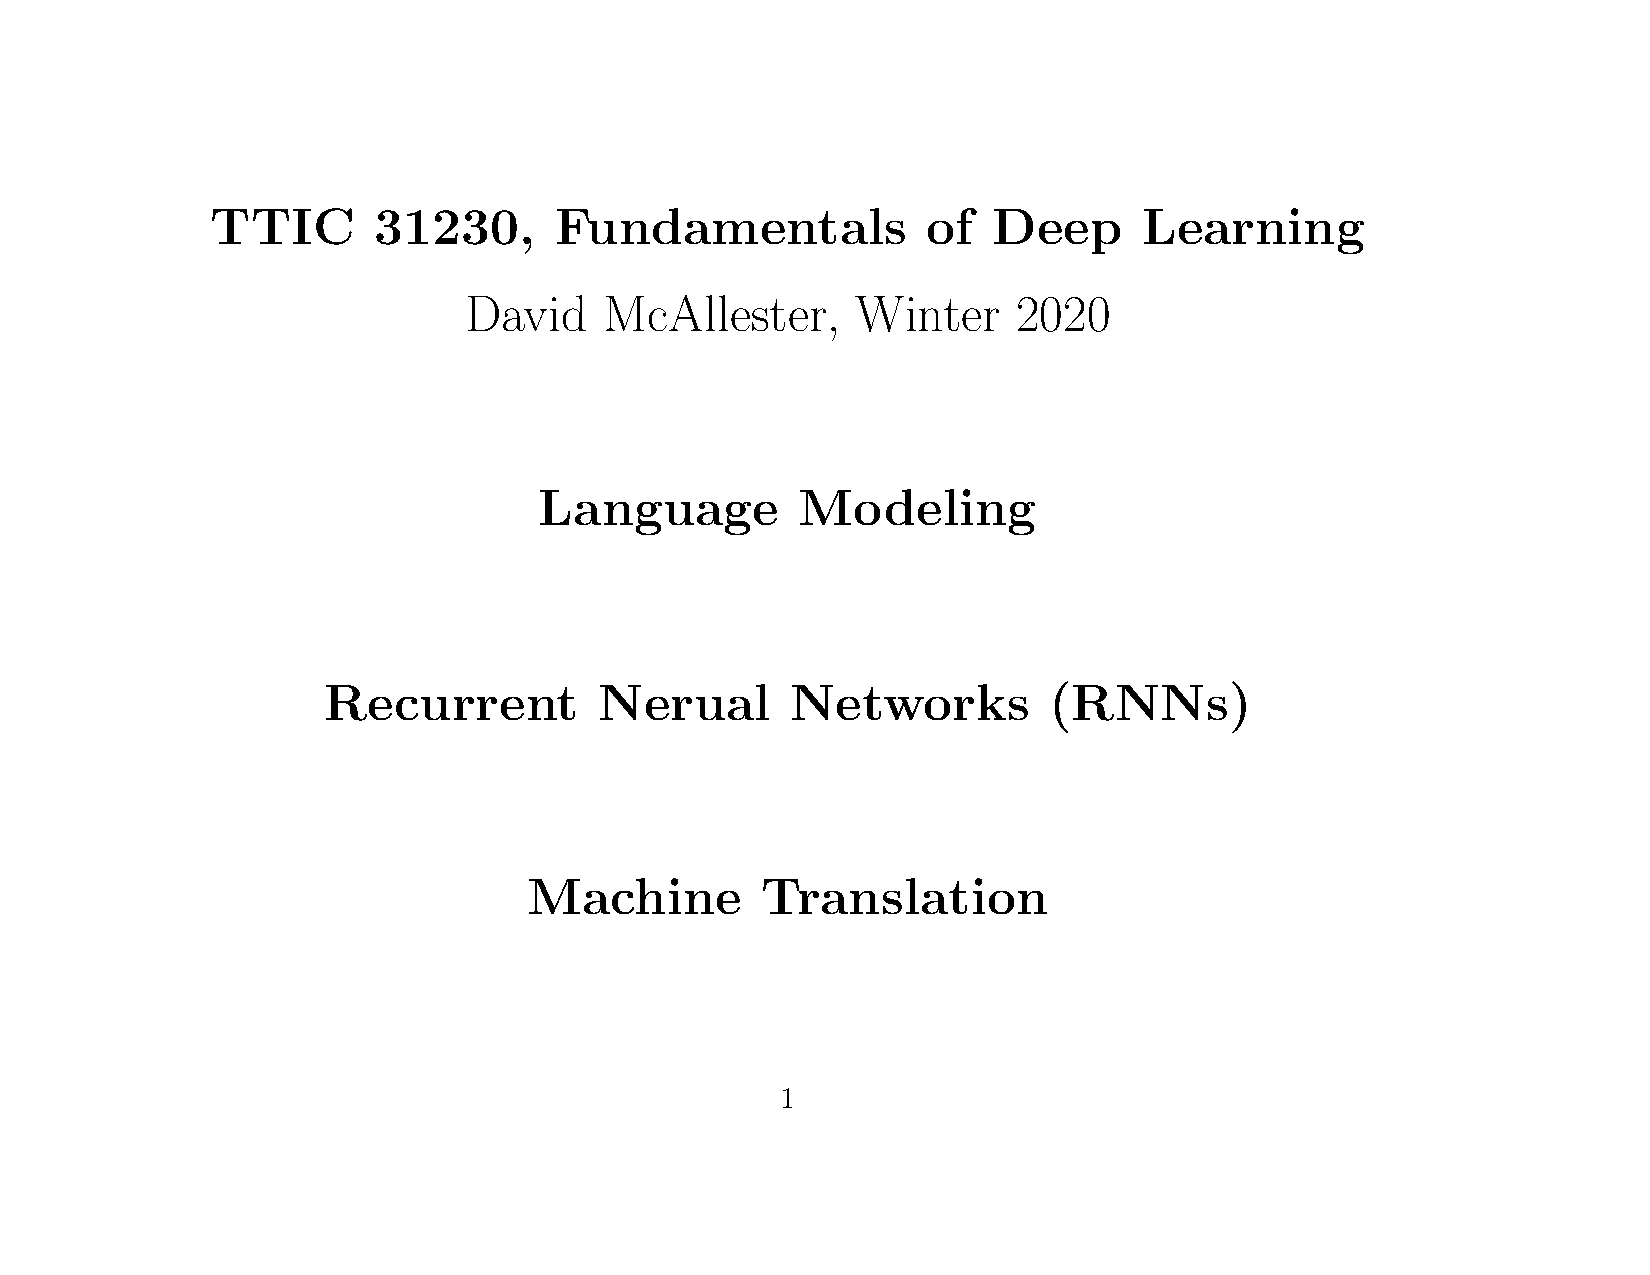
\includegraphics[width=3.5in]{../images/RNN}}
\centerline{{\large [Christopher Olah]}}

\vfill
We would like the RNN to {\color{red} remember and use} information from much earlier inputs.


\vfill
All the issues with depth now occur through time.

\vfill
However, for RNNs {\color{red} at each time step we use the same model parameters.}

\vfill
In CNNs {\color{red} at each layer uses its own model parameters.}

\slide{Skip Connections Through Time}

\centerline{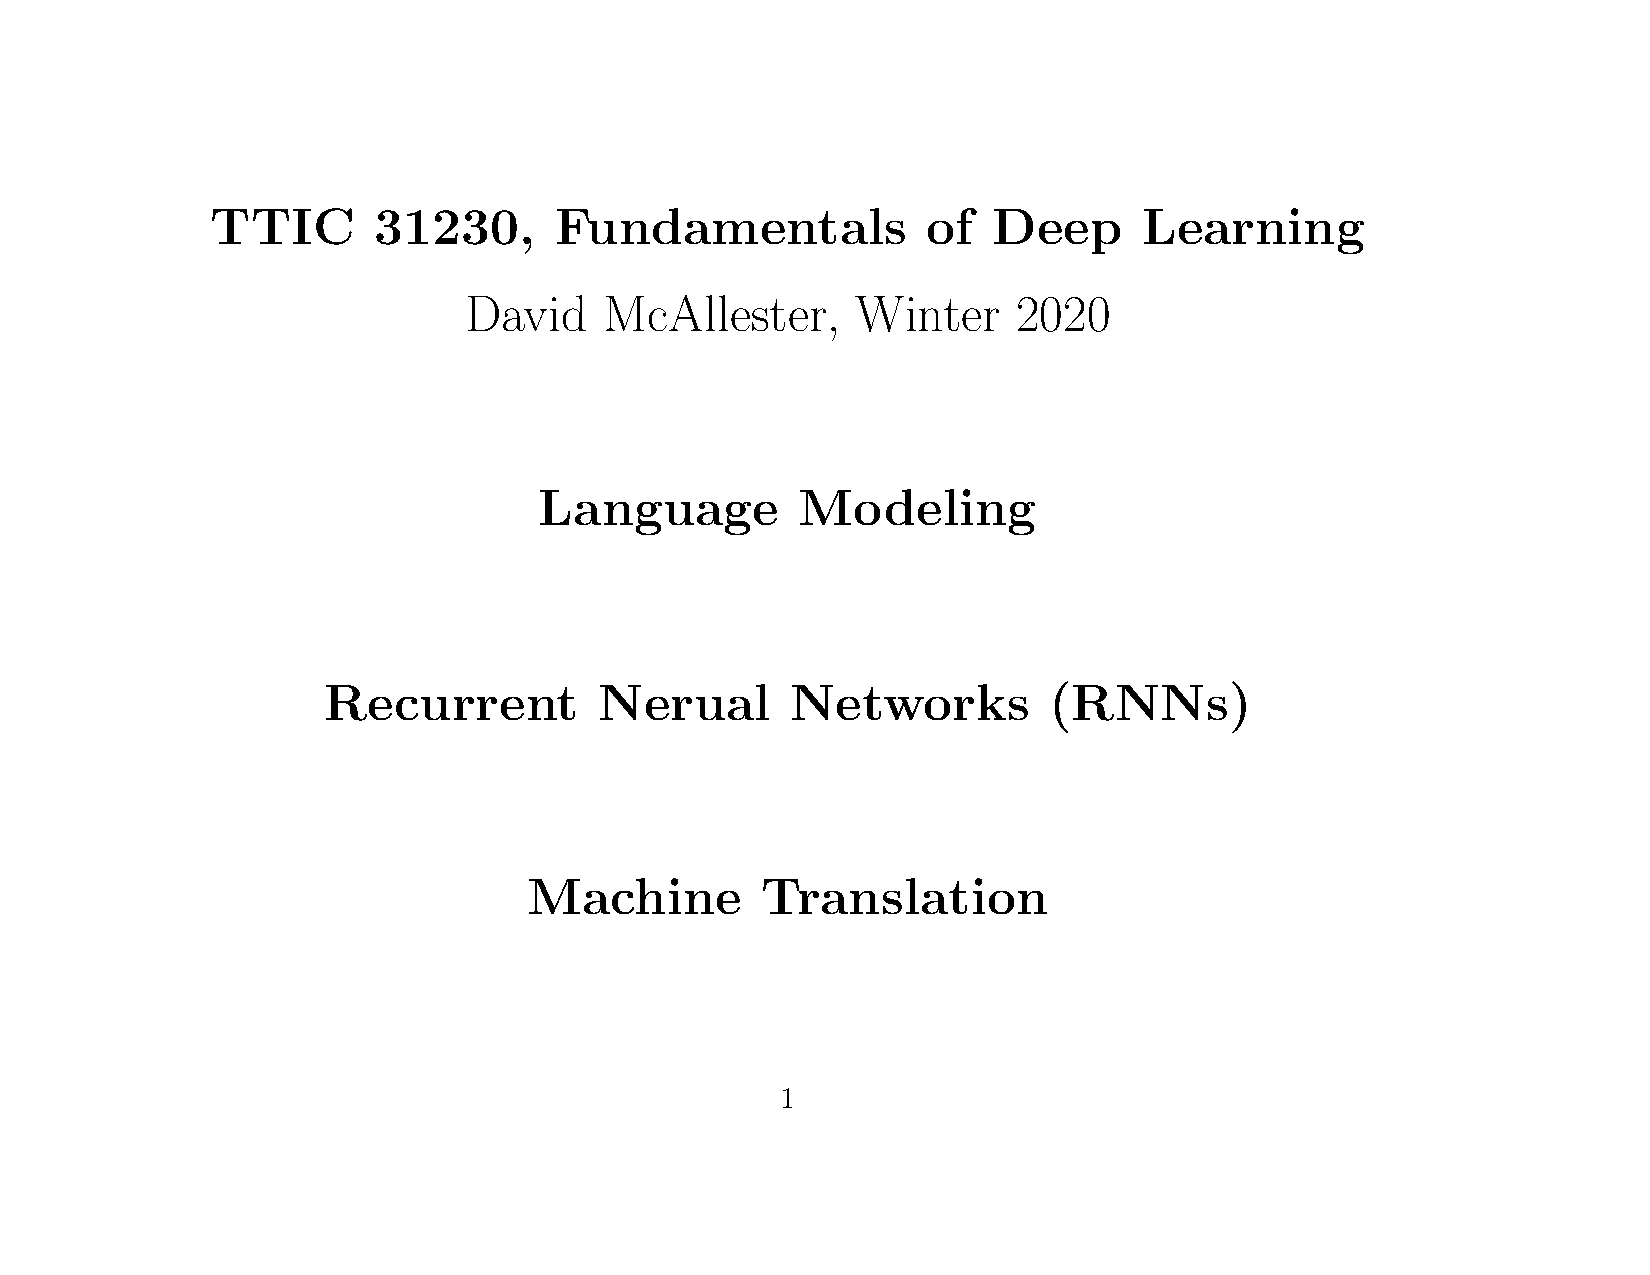
\includegraphics[width=3.5in]{../images/RNN}}
\centerline{{\large [Christopher Olah]}}

\vfill
We would like to add {\color{red} skip connections through time}.

\vfill
However, We have to handle the fact that the same model parameters are used at every time step.


\slideplain{Gated RNNs}

\centerline{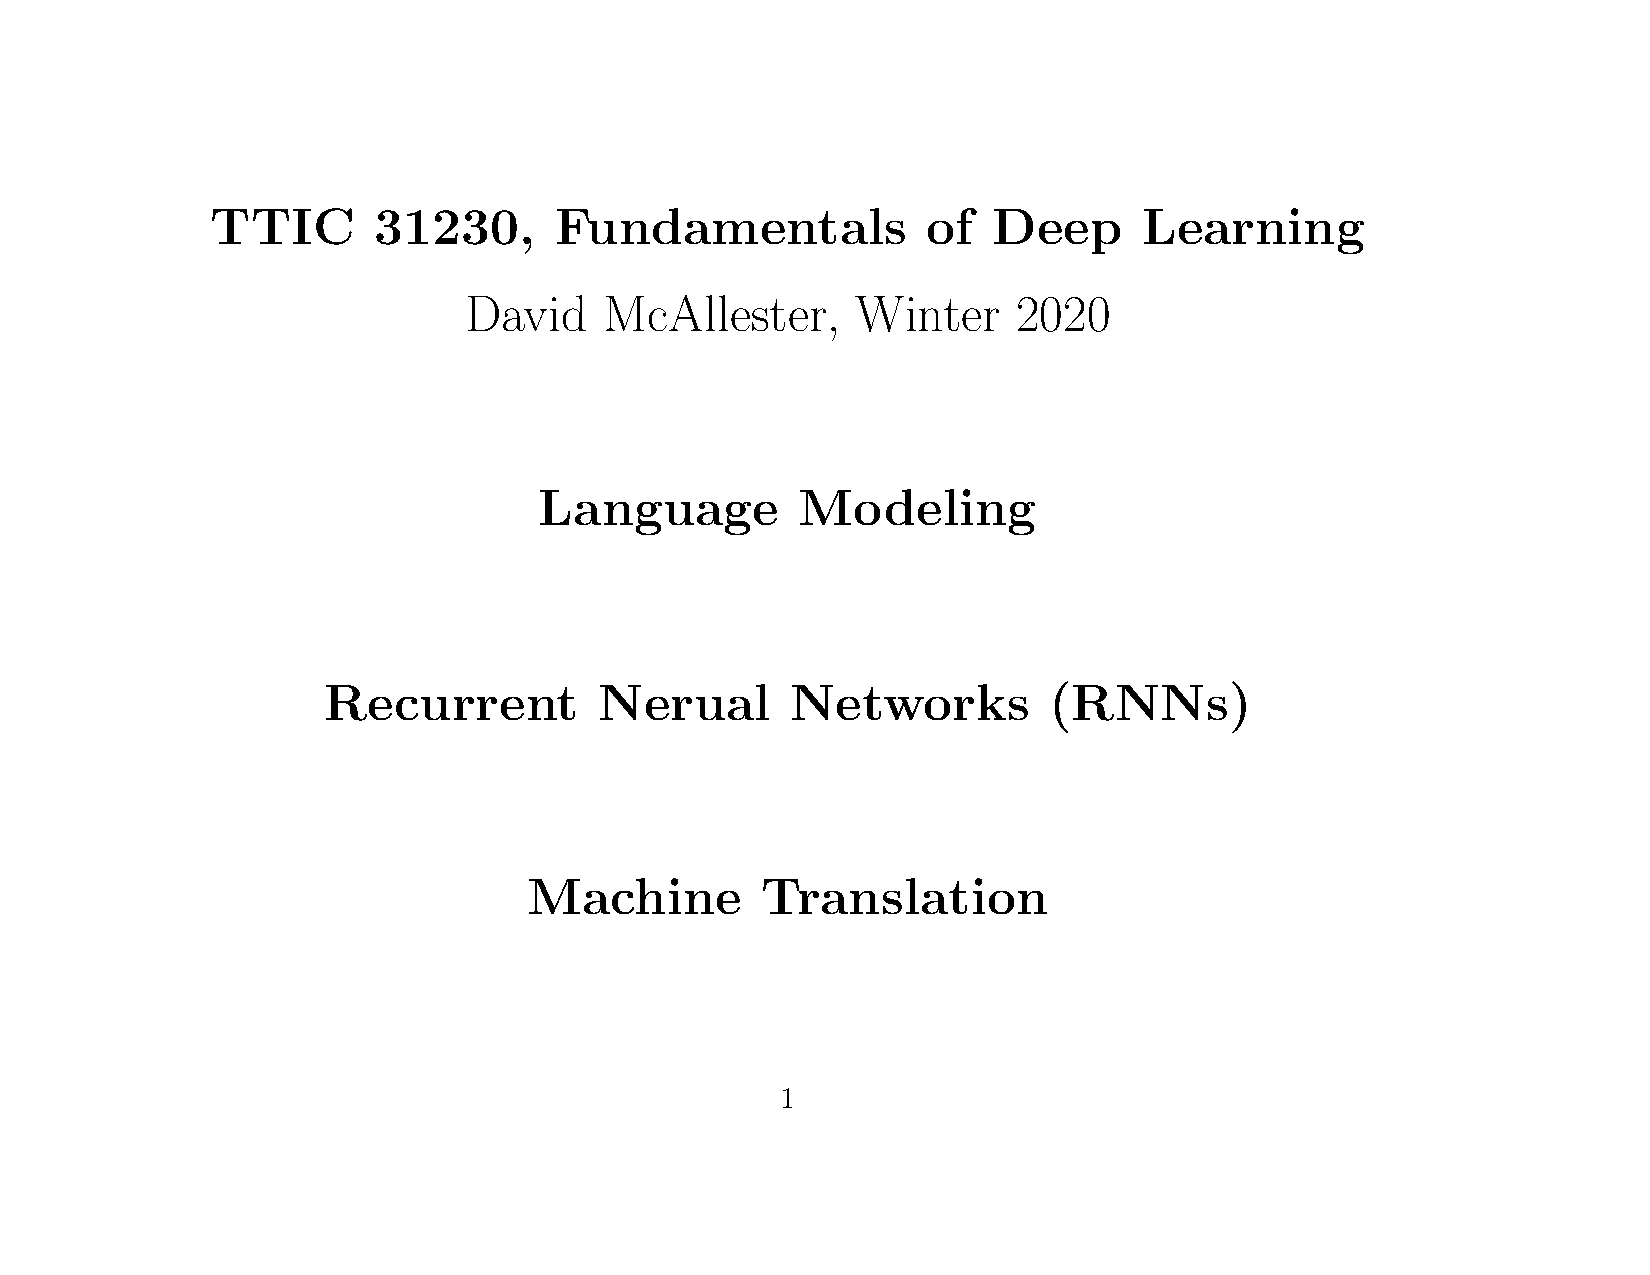
\includegraphics[width=3.5in]{../images/RNN}}
\centerline{{\large [Christopher Olah]}}

$$h[b,t,j] =  {\color{red} G_t[b,t,j]}h[b,t\!-\!1,j] + {\color{red} (1-G[b,t,j])}R[b,t,j]$$

\vfill
Rather than add the diversion $R[b,t,j]$ to $h[b,t\!-\!1,j]$ we take a convex combination determined by a computed ``gate'' $G[b,t,j] \in [0,1]$.

\vfill
For $G[b,t,j] =1$ we pass feature $j$ through unchanged.

For $G[b,t,j] = 0$ we completely replace feature $j$.

\slideplain{Update Gate RNN (UGRNN)}

{\huge
\begin{eqnarray*}
R[b,t,j] & = & \mathrm{tanh}\left(\left(\sum_i\;W^{h,R}[j,i]{\color{red} h[b,t\!-\!1,i]}\right) + \left(\sum_k W^{x,R}[j,k]{\color{red} x[b,t,k]}\right) - B^R[j]\right) \\
\\
G[b,t,j] & = & \sigma\left(\left(\sum_i\;W^{h,G}[j,i]{\color{red} h[b,t\!-\!1,i]}\right) + \left(\sum_k W^{x,G}[j,k]{\color{red} x[b,t,k]}\right) - B^G[j]\right) \\
\\
h[b,t,j] & = & {\color{red} G[b,t,j]}h[b,t\!-\!1,j] + {\color{red} (1-G[b,t,j])}R[b,t,j] \\
\\
{\color{red} \Phi} & {\color{red} =} & {\color{red} (W^{h,R},W^{x,R},B^R,W^{h,G},W^{x,G},B^G)}
\end{eqnarray*}
}

\slide{Hadamard product}

$$h[b,t,j] =  {\color{red} G[b,t,j]}h[b,t\!-\!1,j] + {\color{red} (1-G[b,t,j])}R[b,t,j]$$

\vfill
is sometimes written as

$$h[b,t,J] =  G[b,t,J]{\color{red} \odot} h[b,t\!-\!1,J] + (1-G[b,t,J]){\color{red} \odot} R[b,t,J]$$

\vfill
$\odot$ is the Hadamard product (componentwise product) on vectors.

\slide{Gated Recurrent Unity (GRU) by Cho et al. 2014}

\centerline{\includegraphics[width=4.0in]{../images/GRU}}
\centerline{{\huge [Christopher Olah]}}

\vfill
The right half is a UGRNN.

\vfill
The GRU adds a gating on $h_{t-1}$ before the tanh.

\slide{Long Short Term Memory (LSTM)}
\centerline{\includegraphics[width=3.5in]{../images/LSTM}}
\centerline{{\large [figure: Christopher Olah]}}

\centerline{\Large [LSTM: Hochreiter\&Shmidhuber, 1997]}

\slide{UGRNN vs. GRUs vs. LSTMs}

\vfill
In class projects from previous years, GRUs consistently outperformed LSTMs.

\vfill
A systematic study [Collins, Dickstein and Sussulo 2016] states:

\begin{quotation}
  Our results point to the GRU as being the most learnable of gated RNNs for shallow architectures, followed by the UGRNN.
\end{quotation}

\slide{RNN for a generic CELL Procedure}
As usual, we use capital letter indeces to denote whole tensors or slices and lower case letters to denote particular index values.
\vfill
Procedure $\mathrm{RNN}_\Phi(x(T,I))$

\begin{eqnarray*}
h[0,J] &  = &  \mathrm{CELL}_{\Phi.\mathrm{cell}}(\Phi.\mathrm{init}[J],\;x[0,I]) \\
\mathrm{for}\;t>0\;\;h[t,J] &  =  & \mathrm{CELL}_{\Phi.\mathrm{cell}}(h[t-1,J],\;x[t,I])
\end{eqnarray*}

\vfill
Return $h[T,J]$



\slide{bi-directional RNNS}

\centerline{\includegraphics[width = 3in]{../images/biRNN}}

\begin{eqnarray*}
\vec{h}[T,J] & = & \vec{\mathrm{RNN}}_{\Phi.LR}(x[T,I]) \\
\\
\cev{h}[T,J] & = & \cev{\mathrm{RNN}}_{\Phi.RL}(x[T,I]) \\
\\
\mbox{for}\;t\;\;h[t,2J] & = & \vec{h}[t,J];\cev{h}[t,J]\;\;\mbox{where $x;y$ is vector concatenation}
\end{eqnarray*}

\slide{Multi-Layer RNNs}

\centerline{\includegraphics[width = 2in]{../images/RNNstack}}
\centerline{\large [Figure by Leonardo Araujo dos Santos]}

\begin{eqnarray*}
h[0,T,J] & = & \mathrm{RNN}_{\Phi[0]}(x[T,I]) \\
\\
\mbox{for} \;\ell > 0\;\;h[\ell,T,J] & = & \mathrm{RNN}_{\Phi[\ell]}(h[\ell-1,T,J])
\end{eqnarray*}

Each layer can be bidirectional.

\anaslide{Residual Multi-Layer RNNs}


\begin{eqnarray*}
h[0,T,J] & = & \mathrm{RNN}_{\Phi[0]}(x[T,I]) \\
\\
\mbox{for} \;\ell > 0\;\;h[\ell,T,J] & = & {\color{red} h[\ell-1,T,J] +} \mathrm{RNN}_{\Phi[\ell]}(h[\ell-1,T,J])
\end{eqnarray*}

\vfill
This is used in Google translation.

\slide{}

\centerline{\bf Neural Machine Translation}

\slide{Machine Translation}
%\centerline{\includegraphics[width = 4in]{../images/SeqToSeq}}

%\centerline{\large [Figure from Luong et al.]}

$$w^{\mathrm{in}}_1,\ldots,w^{\mathrm{in}}_{t_{\mathrm{in}}} \Rightarrow w^{\mathrm{out}}_1,\ldots,w^{\mathrm{out}}_{t_{\mathrm{out}}}$$

$$w_{\mathrm{in}}[T_{\mathrm{in}}] \Rightarrow w_{\mathrm{out}}[T_{\mathrm{out}}]$$
\vfill
Translation is a {\bf sequence to sequence} (seq2seq) task.

\vfill
{\bf Sequence to Sequence Learning with Neural Networks}, Sutskever, Vinyals and Le, NIPS 2014, arXiv Sept 10, 2014.

\vfill
We describe a simplification of the paper.

\slide{Machine Translation}

%\centerline{\includegraphics[width = 4in]{../images/SeqToSeq}}

%\centerline{\large [Figure from Luong et al.]}

$$w_{\mathrm{in}}[T_{\mathrm{in}}] \Rightarrow w_{\mathrm{out}}[T_{\mathrm{out}}]$$

\vfill
We define a model

\vfill
$$P_\Phi\left(w_{\mathrm{out}}[T_{\mathrm{out}}]\;|\; w_{\mathrm{in}}[T_\mathrm{in}]\right)$$

\vfill
\begin{eqnarray*}
\Phi^*  & = & \argmin_\Phi\; E_{\mathrm{Pop}} \;-\ln\;P_\Phi(w_{\mathrm{out}}[T_{\mathrm{out}}] \;|\; w_{\mathrm{in}}[T_{\mathrm{in}}]) \\
\\
& = & \argmin_\Phi \; E_{\mathrm{Pop}} \; -\ln P_\Phi(y|x)
\end{eqnarray*}


\slide{A Simple RNN Translation Model}

\vfill
The final state of a right-to-left RNN, $\cev{h}_{\mathrm{in}}[1,J]$, is viewed as a ``thought vector'' representation of the input sentence.

\vfill
We use the input thought vector $\cev{h}_{\mathrm{in}}[1,J]$ as the initial hidden state a left-to-right RNN language model
generating the output sentence.

\vfill
Taking a the thought vector at the beginning of the input sentence facilitates getting a good start in left-to-right modeling of the output.

\slide{Machine Translation Decoding}

We can sample a translation

$$w_t \sim P(w_t\;|\;\cev{h}_{\mathrm{in}}[1,J],\;w_1,\ldots,w_{t-1})$$

\vfill
or we can do greedy decoding

$$w_t = \argmax_{w_t}\; P(w_t\;|\;\cev{h}_{\mathrm{in}}[1,J],\;w_1,\ldots,w_{t-1})$$

\vfill
or we might try maximize total probability.

\begin{eqnarray*}
w_1,\ldots,w_{T_{\mathrm{out}}}
& = & \argmax_{w_1,\ldots,w_{T_{\mathrm{out}}}} \;P_\Phi\left(w_1,\ldots,w_{T_{\mathrm{out}}} \;|\; \cev{h}_{\mathrm{in}}[1,J]\right)
\end{eqnarray*}

\slide{Attention-Based Translation}

{\bf Neural Machine Translation by Jointly Learning to {\color{red} Align} and Translate}
Dzmitry Bahdanau, Kyunghyun Cho, Yoshua Bengio, ICLR 2015 (arXiv Sept. 1, 2014)

\vfill
We describe a simplification of the paper.

\slide{Representing Sentences by Vector Sequences}

The input sentence is now represented by a sequence of vectors.

\vfill
\begin{eqnarray*}
 & & P_\Phi(w_{\mathrm{out}}[T_{\mathrm{out}}] \;|\; w_{\mathrm{in}}[T_{\mathrm{in}}]) \\
 \\
& = & P_{\Phi.\mathrm{out}}(w_{\mathrm{out}}[T_{\mathrm{out}}]\;|\;
{\color{red} M[T_\mathrm{in},J]})
\end{eqnarray*}

\vfill
{\color{red} $M[T_{\mathrm{in}},J]$} is the sequence of hidden states of an RNN
(for some RNN architecture) on the input sentence.

\vfill
{\color{red} $M[t,J]$} is the $t$th hidden vector for the input sentence.

\slide{Attention-Based (Memory-Based) Translation Decoding}



$$h[-1,J] =  M[0,J]$$

\begin{eqnarray*}
P(w_t\;|\;w_0,\cdots,w_{t-1}) & = & \softmax_{w_t}\;e[w_t,I]W^{\mathrm{auto}}[I,J]h[t-1,J] \\
\\
\alpha[t_{\mathrm{in}}]& =& \softmax_{t_\mathrm{in}} \;h[t\!-\!1,J_1]W^{\mathrm{key}}[J_1,J_2]M[t_{\mathrm{in}},J_2]\\
\\
V[J]& = & \sum_{t_{\mathrm{in}}}\;\alpha[t_{\mathrm{in}}]M[t_{\mathrm{in}},J] \\
\\
h[t,J] & = & \mathrm{CELL}_\Phi (h[t-1,J],\;V[J],\;e[w_t,I])
\end{eqnarray*}

\slide{Attention as a Key-Value Memory Mechanism}

Procedure $\mathrm{Lookup}(\mathrm{key}[J],\;M[T,J])$

\bigskip
\begin{eqnarray*}
\alpha[t]& =& \softmax_t \;\mathrm{key}[J]^\top M[t,J]\\
\\
\\
V[J]& =& \sum_t\;\alpha[t]M[t,J]
\end{eqnarray*}

\bigskip
Return $V[J]$



\slideplain{Attention in Image Captioning}

\centerline{\includegraphics[width = 4in]{../images/AttentionInCaptioning1}}
\centerline{Xu et al. ICML 2015}

\slideplain{Greedy Decoding vs. Beam Search}

We would like

\vfill
$$W_{\mathrm{out}}[T_{\mathrm{out}}]^* = \argmax_{W_{\mathrm{out}}[T_{\mathrm{out}}]}
P_\Phi(W_{\mathrm{out}}[T_{\mathrm{out}}] \;|\;W_{\mathrm{in}}[T_{\mathrm{in}}])$$

\vfill
But a greedy algorithm may do well

\vfill
$$w_t = \argmax_w\; P_\Phi(w\;|\;W_{\mathrm{in}}[T_{\mathrm{in}}],\;w_1,\ldots,w_{t-1})$$

\vfill
But these are not the same.

\slide{Example}

``Those apples are good'' vs. ``Apples are good''

\vfill
$$P_\Phi(\mbox{Apples are Good {\tt <eos>}}) > P_\Phi(\mbox{Those apples are good {\tt <eos>}})$$

\vfill
$$P_\Phi(\mbox{Those}|\varepsilon) > P_\Phi(\mbox{Apples}|\varepsilon)$$
    
\slide{Beam Search}

At each time step we maintain a list the $K$ best words and their associated hidden vectors.

\vfill
This can be used to produce a list of $k$ ``best'' decodings which can then be compared to select
the most likely one.

\slideplain{Phrase Based Statistical Machine Translation (SMT)}


Phrase based SMT dominanted machine translation before deep Seq2Seq models.

\vfill
SMT is still used for low resource languages, such as regional African languages, and in unsupervised machine translation.

\slide{Phrase Based Statistical Machine Translation (SMT)}


Step I:   Learn a phrase table --- a set of triples $(p,q,s)$ where

\vfill
\begin{itemize}
\item $p$ is a (short) sequence of source words.
  \vfill
\item $q$ is a (short) sequence of target words.
  \vfill
\item $s$ is a score.
\end{itemize}

\vfill
(``au'', ``to the'', .5) \hfill (``au banque'', ``for the bank'', .01)

\vfill
For a phrase triple $P$ we will write $P.\mathrm{source}$ for the source phrase, $P.\mathrm{target}$ for the target phrase, and $P.\mathrm{score}$ for the score.

\slide{Derivations}

Consider an input sentence $x$ of length $T$.

\vfill
We will write $x[s:t]$ for the substring $x[s]$, $\ldots$, $x[t-1]$.

\vfill
A derivation $d$ from $x$ is a sequence $(P_1,s_1,t_1,)$, $\ldots$, $(P_K,s_K,t_K)$ where $P_k.\mathrm{source} = x[s_k:t_k]$.

\vfill
The substrings $x[s_k:t_k]$ should be disjoint and ``cover'' $x$.

\vfill
For $d = [(P_1,s_1,t_1,)$, $\ldots$, $(P_L,s_K,t_K)]$ we define

$$ y(d) \equiv P_1.\mathrm{target}\;\cdots P_K.\mathrm{target}$$

\vfill
We let $D(x)$ be the set of derivations from $x$.

\slide{Scoring}

For $d \in D(x)$ we define a score $s(d)$

\vfill
$$s(d) = \alpha \ln P_\mathrm{LM}(y(d)) + \beta \sum_k P_k.\mathrm{score} + \gamma \;\mathrm{distortion}(d)$$

\vfill
where $P_{\mathrm{LM}}(y)$ is the probability assigned to string $y$ under a language model for the target language

\vfill
and $\mathrm{distortion}(d)$ is a measure of consistency of word ordering between source and target strings as defined by
the indeces $(s_1,t_1)$, $\ldots$, $(s_K,t_K)$.

\slide{Translation}

\begin{eqnarray*}
  y(x) & = & y(d^*(x)) \\
  \\
  \\
  \\
  d^*(x) & = & \argmax_{d \in D(x)} \;s(d)
\end{eqnarray*}

\slide{END}
}
\end{document}
